\documentclass{article}


% if you need to pass options to natbib, use, e.g.:
%     \PassOptionsToPackage{numbers, compress}{natbib}
% before loading neurips_2023


% ready for submission
% \usepackage{neurips_2023}


% to compile a preprint version, e.g., for submission to arXiv, add add the
% [preprint] option:
\usepackage[preprint]{neurips_2023}


% to compile a camera-ready version, add the [final] option, e.g.:
%     \usepackage[final]{neurips_2023}


% to avoid loading the natbib package, add option nonatbib:
%    \usepackage[nonatbib]{neurips_2023}


\usepackage[utf8]{inputenc} % allow utf-8 input
\usepackage[T1]{fontenc}    % use 8-bit T1 fonts
\usepackage{hyperref}       % hyperlinks
\usepackage{url}            % simple URL typesetting
\usepackage{booktabs}       % professional-quality tables
\usepackage{amsfonts}       % blackboard math symbols
\usepackage{nicefrac}       % compact symbols for 1/2, etc.
\usepackage{microtype}      % microtypography
\usepackage{xcolor}         % colors

\usepackage{amsmath}
\usepackage{amsthm}
\usepackage{graphicx}

% Bibliography
\bibliographystyle{plainnat}
\setcitestyle{numbers,square,comma}

% Numbered Environments:
\newtheorem{definition}{Definition}[section]


\title{ECCCos from the Black Box: Letting Models speak for Themselves}


% The \author macro works with any number of authors. There are two commands
% used to separate the names and addresses of multiple authors: \And and \AND.
%
% Using \And between authors leaves it to LaTeX to determine where to break the
% lines. Using \AND forces a line break at that point. So, if LaTeX puts 3 of 4
% authors names on the first line, and the last on the second line, try using
% \AND instead of \And before the third author name.


\author{%
  Patrick Altmeyer\thanks{Use footnote for providing further information
    about author (webpage, alternative address)---\emph{not} for acknowledging
    funding agencies.} \\
  Faculty of Electrical Engineering, Mathematics and Computer Science\\
  Delft University of Technology\\
  2628 XE Delft, The Netherlands \\
  \texttt{p.altmeyer@tudelft.nl} \\
  % examples of more authors
  % \And
  % Coauthor \\
  % Affiliation \\
  % Address \\
  % \texttt{email} \\
  % \AND
  % Coauthor \\
  % Affiliation \\
  % Address \\
  % \texttt{email} \\
  % \And
  % Coauthor \\
  % Affiliation \\
  % Address \\
  % \texttt{email} \\
  % \And
  % Coauthor \\
  % Affiliation \\
  % Address \\
  % \texttt{email} \\
}


\begin{document}


\maketitle


\begin{abstract}
  We propose Conformal Counterfactual Explanations: an effortless and rigorous way to produce plausible and conformal Counterfactual Explanations for Black Box Models using Conformal Prediction. To address the need for plausible explanations, existing work has primarily relied on surrogate models to learn the data-generating process. This effectively reallocates the task of learning realistic representations of the data from the model itself to the surrogate. Consequently, the generated explanations may look plausible to humans but not necessarily conform with the behaviour of the Black Box Model. We formalise this notion through the introduction of new evaluation measures. In order to still address the need for plausibility, we build on a recent approach that works by minimizing predictive model uncertainty. Using differentiable Conformal Prediction, we relax the previous assumption that the Black Box Model can produce predictive uncertainty estimates.
\end{abstract}

\section{Introduction}\label{intro}

Counterfactual Explanations are a powerful, flexible and intuitive way to not only explain Black Box Models but also enable affected individuals to challenge them through the means of Algorithmic Recourse. Instead of opening the black box, Counterfactual Explanations work under the premise of strategically perturbing model inputs to understand model behaviour \citep{wachter2017counterfactual}. Intuitively speaking, we generate explanations in this context by asking simple what-if questions of the following nature: `Our credit risk model currently predicts that this individual's credit profile is too risky to offer them a loan. What if they reduced their monthly expenditures by 10\%? Will our model then predict that the individual is credit-worthy'? 

This is typically implemented by defining a target outcome $\mathbf{y}^* \in \mathcal{Y}$ for some individual $\mathbf{x} \in \mathcal{X}=\mathbb{R}^D$ described by $D$ attributes, for which the model $M_{\theta}:\mathcal{X}\mapsto\mathcal{Y}$ initially predicts a different outcome: $M_{\theta}(\mathbf{x})\ne \mathbf{y}^*$. Counterfactuals are then searched by minimizing a loss function that compares the predicted model output to the target outcome: $\text{yloss}(M_{\theta}(\mathbf{x}),\mathbf{y}^*)$. Since Counterfactual Explanations (CE) work directly with the Black Box Model, valid counterfactuals always have full local fidelity by construction \citep{mothilal2020explaining}. Fidelity is defined as the degree to which explanations approximate the predictions of the Black Box Model. This is arguably one of the most important evaluation metrics for model explanations, since any explanation that explains a prediction not actually made by the model is useless \citep{molnar2020interpretable}. 

In situations where full fidelity is a requirement, CE therefore offers a more appropriate solution to Explainable Artificial Intelligence (XAI) than other popular approaches like LIME \citep{ribeiro2016why} and SHAP \citep{lundberg2017unified}, which involve local surrogate models. But even full fidelity is not a sufficient condition for ensuring that an explanation adequately describes the behaviour of a model. That is because two very distinct explanations can both lead to the same model prediction, especially when dealing with heavily parameterized models:

\begin{quotation}
  […] deep neural networks are typically very underspecified by the available data, and […] parameters [therefore] correspond to a diverse variety of compelling explanations for the data.
  --- \citet{wilson2020case}
\end{quotation}

When people talk about Black Box Models, this is usually the type of model they have in mind. 

In the context of CE, the idea that no two explanations are the same arises almost naturally. Even the baseline approach proposed by \citet{wachter2017counterfactual} can yield a diverse set of explanations if counterfactuals are initialised randomly. This multiplicity of explanations has not only been acknowledged in the literature but positively embraced: since individuals seeking Algorithmic Recourse (AR) have unique preferences,~\citet{mothilal2020explaining}, for example, have prescribed \textit{diversity} as an explicit goal for counterfactuals. More generally, the literature on CE and AR has brought forward a myriad of desiderata for explanations, which we will discuss in more detail in the following section.

\section{From Adversarial Examples to Plausible Explanations}\label{background}

In this section, we provide some background on Counterfactual Explanations and our motivation for this work. To start off, we briefly introduce the methodology uncerlying most state-of-the-art (SOTA) counterfactual generators.

While Counterfactual Explanations can be generated for arbitrary regression models \citep{spooner2021counterfactual}, existing work has primarily focused on classification problems. Let $\mathcal{Y}=(0,1)^K$ denote the one-hot-encoded output domain with $K$ classes. Then most SOTA counterfactual generators rely on gradient descent to optimize different flavours of the following counterfactual search objective:

\begin{equation} \label{eq:general}
\begin{aligned}
\mathbf{Z}^\prime &= \arg \min_{\mathbf{Z}^\prime \in \mathcal{Z}^M} \left\{  {\text{yloss}(M_{\theta}(f(\mathbf{Z}^\prime)),\mathbf{y}^*)}+ \lambda {\text{cost}(f(\mathbf{Z}^\prime)) }  \right\} 
\end{aligned} 
\end{equation}

Here $\text{yloss}$ denotes the primary loss function already introduced above and $\text{cost}$ is either a single penalty or a collection of penalties that are used to impose constraints through regularization. Following the convention in \citet{altmeyer2023endogenous} we use $\mathbf{Z}^\prime=\{ \mathbf{z}_m\}_M$ to denote the vector $M$-dimensional array of counterfactual states. This is to explicitly account for the fact that we can generate multiple counterfactuals $M$, as with DiCE \citep{mothilal2020explaining}, and may choose to traverse a latent representation $\mathcal{Z}$ of the feature space $\mathcal{X}$, as we will discuss further below. 

Solutions to Equation~\ref{eq:general} are considered valid as soon as the predicted label matches the target label. A stripped-down counterfactual explanation is therefore little different from an adversarial example. In Figure~\ref{fig:adv}, for example, we have the baseline approach proposed in \citet{wachter2017counterfactual} to MNIST data (centre panel). This approach solves Equation~\ref{eq:general} through gradient-descent in the feature space with a penalty for the distance between the factual $\mathbf{x}$ and the counterfactual $\mathbf{x}^{\prime}$. The underlying classifier $M_{\theta}$ is a simple Multi-Layer Perceptron (MLP) with good test accuracy. For the generated counterfactual $\mathbf{x}^{\prime}$ the model predicts the target label with high confidence (centre panel in Figure~\ref{fig:adv}). The explanation is valid by definition, even though it looks a lot like an Adversarial Example \citep{goodfellow2014explaining}. \citet{schut2021generating} make the connection between Adversarial Examples and Counterfactual Explanations explicit and propose using a Jacobian-Based Saliency Map Attack (JSMA) to solve Equation~\ref{eq:general}. They demonstrate that this approach yields realistic and sparse counterfactuals for Bayesian, adversarially robust classifiers. Applying their approach to our simple MNIST classifier does not yield a realistic counterfactual but this one, too, is valid (right panel in Figure~\ref{fig:adv}). 

The crucial difference between Adversarial Examples (AE) and Counterfactual Explanations is one of intent. While an AE is intended to go unnoticed, a CE should have certain desirable properties. The literature has made this explicit by introducing various so-called \textit{desiderata}. To properly serve both AI practitioners and individuals affected by AI decision-making systems, counterfactuals should be sparse, proximate~\citep{wachter2017counterfactual}, actionable~\citep{ustun2019actionable}, diverse~\citep{mothilal2020explaining}, plausible~\citep{joshi2019realistic,poyiadzi2020face,schut2021generating}, robust~\citep{upadhyay2021robust,pawelczyk2022probabilistically,altmeyer2023endogenous} and causal~\citep{karimi2021algorithmic} among other things. 

Researchers have come up with various ways to meet these desiderata, which have been extensively surveyed and evaluated in various studies~\citep{verma2020counterfactual,karimi2020survey,pawelczyk2021carla,artelt2021evaluating,guidotti2022counterfactual}. Perhaps unsurprisingly, the different desiderata are often positively correlated. For example, \citet{artelt2021evaluating} find that plausibility typically also leads to improved robustness. Similarly, plausibility has also been connected to causality in the sense that plausible counterfactuals respect causal relationships \citep{mahajan2020preserving}. 

Arguably, the plausibility of counterfactuals has been among the primary concerns and some have focused explicitly on this goal. \citet{joshi2019realistic}, for example, were among the first to suggest that instead of searching counterfactuals in the feature space $\mathcal{X}$, we can instead traverse a latent embedding $\mathcal{Z}$ that implicitly codifies the data generating process (DGP) of $\mathbf{x}\sim\mathcal{X}$. To learn the latent embedding, they introduce a surrogate model. In particular, they propose to use the latent embedding of a Variational Autoencoder (VAE) trained to generate samples $\mathbf{x}^* \leftarrow \mathcal{G}(\mathbf{z})$ where $\mathcal{G}$ denotes the decoder part of the VAE. Provided the surrogate model is well-trained, their proposed approach ---REVISE--- can yield compelling counterfactual explanations like the one in the centre panel of Figure~\ref{fig:vae}. 

Others have proposed similar approaches. \citet{dombrowski2021diffeomorphic} traverse the base space of a normalizing flow to solve Equation~\ref{eq:general}, essentially relying on a different surrogate model for the generative task. \citet{poyiadzi2020face} use density estimators ($\hat{p}: \mathcal{X} \mapsto [0,1]$) to constrain the counterfactual paths. \citet{karimi2021algorithmic} argue that counterfactuals should comply with the causal model that generates the data. All of these different approaches share a common goal: ensuring that the generated counterfactuals comply with the true and unobserved DGP. To summarize this broad objective, we propose the following definition:

\begin{definition}[Plausible Counterfactuals]
  \label{def:plausible}
  Let $\mathcal{X}|\mathbf{y}^*$ denote the true conditional distribution of samples in the target class $\mathbf{y}^*$. Then for $\mathbf{x}^{\prime}$ to be considered a plausible counterfactual, we need: $\mathbf{x}^{\prime} \sim \mathcal{X}|\mathbf{y}^*$.
\end{definition}

Note that Definition~\ref{def:plausible} is consistent with the notion of plausible counterfactual paths, since we can simply apply it to each counterfactual state along the path.

Surrogate models offer an obvious solution to achieve this objective. Unfortunately, surrogates also introduce a dependency: the generated explanations no longer depend exclusively on the Black Box Model itself, but also on the surrogate model. This is not necessarily problematic if the primary objective is not to explain the behaviour of the model but to offer recourse to individuals affected by it. It may become problematic even in this context if the dependency turns into a vulnerability. To illustrate this point, we have used REVISE \citep{joshi2019realistic} with an underfitted VAE to generate the counterfactual in the right panel of Figure~\ref{fig:vae}: in this case, the decoder step of the VAE fails to yield plausible values ($\{\mathbf{x}^{\prime} \leftarrow \mathcal{G}(\mathbf{z})\} \not\sim \mathcal{X}|\mathbf{y}^*$) and hence the counterfactual search in the learned latent space is doomed.

\begin{figure}
  \centering
  \begin{minipage}[t]{0.45\textwidth}
    \centering
    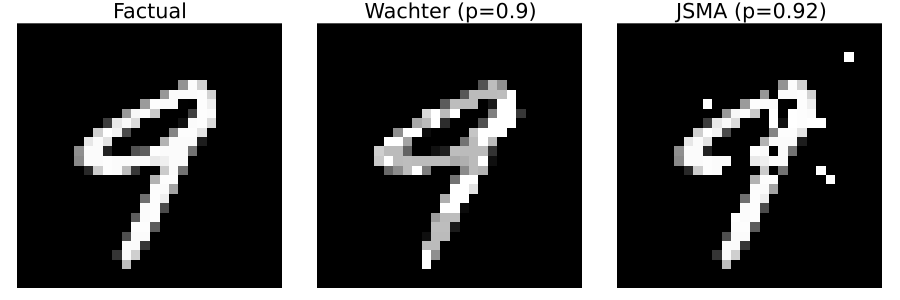
\includegraphics[width=\textwidth]{../www/you_may_not_like_it.png}
    \caption{You may not like it, but this is what stripped-down counterfactuals look like. Counterfactuals for turning an 8 (eight) into a 3 (three): original image (left); counterfactual produced using \citet{wachter2017counterfactual} (centre); and a counterfactual produced using JSMA-based approach introduced by \citep{schut2021generating}.}\label{fig:adv}
  \end{minipage}\hfill
  \begin{minipage}[t]{0.45\textwidth}
    \centering
    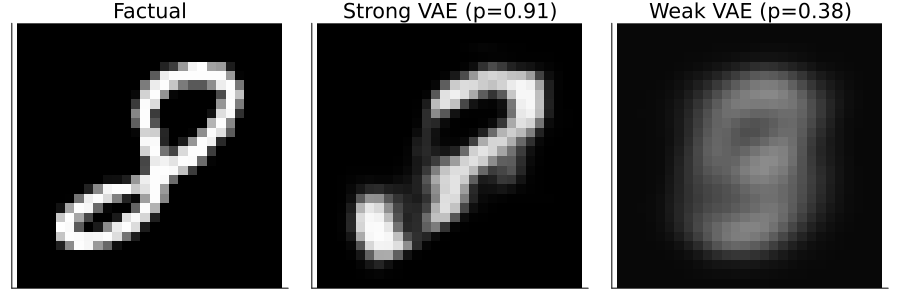
\includegraphics[width=\textwidth]{../www/surrogate_gone_wrong.png}
    \caption{Using surrogates can improve plausibility, but also increases vulnerability. Counterfactuals for turning an 8 (eight) into a 3 (three): original image (left); counterfactual produced using REVISE \citep{joshi2019realistic} with a well-specified surrogate (centre); and a counterfactual produced using REVISE \citep{joshi2019realistic} with a poorly specified surrogate (right).}\label{fig:vae}
  \end{minipage}
\end{figure}

\section{Evaluating the Faithfulness of Counterfactuals}\label{conformity}

In Section~\ref{background} we explained that Counterfactual Explanations work directly with Black Box Model, so fidelity is not a concern. This may explain why research has primarily focused on other desiderata, most notably plausibility (Definition~\ref{def:plausible}). Enquiring about the plausibility of a counterfactual essentially boils down to the following question: `Is this counterfactual consistent with the underlying data'? To introduce this section, we posit a related, slightly more nuanced question: `Is this counterfactual consistent with what the model has learned about the underlying data'? We will argue that fidelity is not a sufficient evaluation measure to answer this question and propose a novel way to assess if explanations conform with model behaviour. Finally, we will introduce a framework for Conformal Counterfactual Explanations, that reconciles the notions of plausibility and model conformity. 

\subsection{From Fidelity to Model Conformity}

The word \textit{fidelity} stems from the Latin word `fidelis', which means `faithful, loyal, trustworthy' \citep{mw2023fidelity}. As we explained in Section~\ref{background}, model explanations are considered faithful if their corresponding predictions coincide with the predictions made by the model itself. Since this definition of faithfulness is not useful in the context of Counterfactual Explanations, we propose an adapted version: 

\begin{definition}[Conformal Counterfactuals]
  \label{def:conformal}
  Let $\mathcal{X}_{\theta}|\mathbf{y}^* = p_{\theta}(x|\mathbf{y}^*)$ denote the conditional distribution of $\mathbf{x}$ in the target class $\mathbf{y}^*$, where $\theta$ denotes the parameters of model $M_{\theta}$. Then for $\mathbf{x}^{\prime}$ to be considered a conformal counterfactual, we need: $\mathbf{x}^{\prime} \sim \mathcal{X}_{\theta}|\mathbf{y}^*$.
\end{definition}

In words, conformal counterfactuals conform with what the predictive model has learned about the input data $\mathbf{x}$. Since this definition works with distributional properties, it explicitly accounts for the multiplicity of explanations we discussed earlier. Except for the posterior conditional distribution $p_{\theta}(\mathbf{x}|\mathbf{y}^*)$, we already have access to all the ingredients in Definition~\ref{def:conformal}.

How can we quantify $p_{\theta}(\mathbf{x}|\mathbf{y}^*)$? After all, the predictive model $M_{\theta}$ was trained to discriminate outputs conditional on inputs, which is a different conditional distribution: $p_{\theta}(\mathbf{y}|\mathbf{x})$. Learning the distribution over inputs $p_{\theta}(\mathbf{x}|\mathbf{y}^*)$ is a generative task that $M_{\theta}$ was not explicitly trained for. In the context of Counterfactual Explanations, it is the task that existing approaches have reallocated from the model itself to a surrogate. 

Fortunately, recent work by \citet{grathwohl2020your} on Energy Based Models (EBM) has pointed out that there is a `generative model hidden within every standard discriminative model'. The authors show that we can draw samples from the posterior conditional distribution $p_{\theta}(\mathbf{x}|\mathbf{y})$ using Stochastic Gradient Langevin Dynamics (SGLD). In doing so, it is possible to train classifiers jointly for the discriminative task using standard cross-entropy and the generative task using SGLD. They demonstrate empirically that among other things this improves predictive uncertainty quantification for discriminative models. 

To see how their proposed conditional sampling strategy can be applied in our context, note that if we fix $\mathbf{y}$ to our target value $\mathbf{y}^*$, we can sample from $p_{\theta}(\mathbf{x}|\mathbf{y}^*)$ using SGLD as follows, 

\begin{equation}\label{eq:sgld}
  \begin{aligned}
    \mathbf{x}_{j+1} &\leftarrow \mathbf{x}_j - \frac{\epsilon^2}{2} \mathcal{E}(\mathbf{x}_j|\mathbf{y}^*) + \epsilon \mathbf{r}_j, && j=1,...,J
  \end{aligned}
\end{equation}

where $\mathbf{r}_j \sim \mathcal{N}(\mathbf{0},\mathbf{I})$ is the stochastic term and the step-size $\epsilon$ is typically polynomially decayed. The term $\mathcal{E}(\mathbf{x}_j|\mathbf{y}^*)$ denotes the energy function where as in \citep{grathwohl2020your} we use $\mathcal{E}(\mathbf{x}_j|\mathbf{y}^*)=-M_{\theta}(\mathbf{x}_j)[\mathbf{y}^*]$, that is the negative logit corresponding to the target class label $\mathbf{y}^*$.

While $\mathbf{x}_J$ is only guaranteed to distribute as $p_{\theta}(\mathbf{x}|\mathbf{y}^*)$ if $\epsilon \rightarrow 0$ and $J \rightarrow \infty$, the bias introduced for a small finite $\epsilon$ is negligible in practice \citep{murphy2023probabilistic,grathwohl2020your}. While \citet{grathwohl2020your} use Equation~\ref{eq:sgld} during training, we are interested in applying the conditional sampling procedure in a post hoc fashion to any standard discriminative model. Generating multiple samples in this manner yields an empirical distribution $\hat{\mathcal{X}}_{\theta}|\mathbf{y}^*$, which we can use to assess if a given counterfactual $\mathbf{x}^{\prime}$ conforms with the model $M_{\theta}$ (Definition~\ref{def:conformal}). 

\textbf{TBD}

\begin{itemize}
  \item What exact sampler do we use? ImproperSGLD as in \citet{grathwohl2020your} seems to work best.
\end{itemize}

\subsection{Evaluation Measures}\label{evaluation}

Above we have defined plausibility (\ref{def:plausible}) and conformity (\ref{def:conformal}) for Counterfactual Explanations. In this subsection, we introduce evaluation measures that facilitate a quantitative evaluation of counterfactuals for these objectives. 

Firstly, in order to assess the plausibility of counterfactuals we adapt the implausibility metric proposed in \citet{guidotti2022counterfactual}. The authors propose to evaluate plausibility in terms of the distance of the counterfactual $\mathbf{x}^{\prime}$ from its nearest neighbour in the target class $\mathbf{y}^*$: the smaller this distance, the more plausible the counterfactual. Instead of focusing only on the nearest neighbour of $\mathbf{x}^{\prime}$, we suggest computing the average over distances from multiple (possibly all) observed instances in the target class. Formally, for a single counterfactual, we have:

\begin{equation}\label{eq:impl}
  \begin{aligned}
    \text{impl} = \frac{1}{\lvert\mathbf{x} \in \mathcal{X}|\mathbf{y}^*\rvert} \sum_{\mathbf{x} \in \mathcal{X}|\mathbf{y}^*} \text{dist}(\mathbf{x}^{\prime},\mathbf{x})
  \end{aligned}
\end{equation}

This measure is straightforward to compute and should be less sensitive to outliers in the target class than the one based on the nearest neighbour. It also gives rise to a very similar evaluation measure for conformity. We merely swap out the subsample of individuals in the target class for the empirical distribution of generated conditional samples:

\begin{equation}\label{eq:conf}
  \begin{aligned}
    \text{conf} = \frac{1}{\lvert\mathbf{x} \in \mathcal{X}_{\theta}|\mathbf{y}^*\rvert} \sum_{\mathbf{x} \in \mathcal{X}_{\theta}|\mathbf{y}^*} \text{dist}(\mathbf{x}^{\prime},\mathbf{x})
  \end{aligned}
\end{equation}

As noted by \citet{guidotti2022counterfactual}, these distance-based measures are simplistic and more complex alternative measures may ultimately be more appropriate for the task. For example, we considered using statistical divergence measures instead. This would involve generating not one but many counterfactuals and comparing the generated empirical distribution to the target distributions in Definitions~\ref{def:plausible} and~\ref{def:conformal}. While this approach is potentially more rigorous, generating enough counterfactuals is not always practical. 

\section{A Framework for Conformal Counterfactual Explanations}\label{cce}

Now that we have a framework for evaluating Counterfactual Explanations in terms of their plausibility and conformity, we are interested in finding a way to generate counterfactuals that are as plausible and conformal as possible. We hypothesize that a narrow focus on plausibility may come at the cost of reduced conformity. Using a surrogate model for the generative task, for example, may improve plausibility but inadvertently yield counterfactuals that are more consistent with the surrogate than the Black Box Model itself. We suggest that one way to ensure model conformity is to rely strictly on the model itself. In this section, we introduce a novel framework that meets this requirement, works under minimal assumptions and does not impede the plausibility objective: Conformal Counterfactual Explanations.

\subsection{Plausible Counterfactuals through Minimal Uncertainty}

Our proposed methodology is built on the findings presented in~\citet{schut2021generating}. The authors demonstrate that it is not only possible but remarkably easy to generate plausible counterfactuals for Black Box Models that provide predictive uncertainty estimates. Their proposed algorithm solves Equation~\ref{eq:general} by greedily applying JSMA in the feature space with standard cross-entropy loss and no penalty at all. They show that this is equivalent to minimizing predictive uncertainty and hence yields counterfactuals for which the model $M_{\theta}$ predicts the target label $\mathbf{y}^*$ with high confidence. Provided the model is well-calibrated, these counterfactuals are plausible which the authors demonstrate empirically through benchmarks \citep{schut2021generating}.

Unfortunately, this idea hinges on the crucial assumption that the Black Box Model provides predictive uncertainty estimates. The authors argue that in light of rapid advances in Bayesian Deep Learning (DL), this assumption is overall less costly than the engineering overhead induced by using surrogate models. This is even more true today, as recent work has put Laplace Approximation back on the map for truly effortless Bayesian DL \citep{immer2020improving,daxberger2021laplace,antoran2023sampling}. Nonetheless, the need for Bayesian methods may be too restrictive in some cases. 

In looking for ways to lift that restriction, we found a promising alternative candidate for predictive uncertainty quantification (UQ) that we will briefly introduce next: Conformal Prediction. 

\subsection{Conformal Prediction}

Conformal Prediction (CP) is a scalable and statistically rigorous approach to predictive UQ that works under minimal distributional assumptions \citep{angelopoulos2021gentle}. It has recently gained popularity in the Machine Learning community \citep{angelopoulos2021gentle,manokhin2022awesome}. Crucially for our intended application, CP is model-agnostic and can be applied at test time. This allows us to relax the assumption that the Black Box Model needs to learn to generate predictive uncertainty estimates during training. In other words, CP promises to provide a way to generate plausible counterfactuals for any standard discriminative model without the need for surrogate models. 

Intuitively, CP works under the premise of turning heuristic notions of uncertainty into rigorous uncertainty estimates by repeatedly sifting through the data. It can be used to generate prediction intervals for regression models and prediction sets for classification models \citep{altmeyer2022conformal}. Since the literature on CE and AR is typically concerned with classification problems, we focus on the latter. A particular variant of CP called Split Conformal Prediction (SCP) is well-suited for our purposes because it imposes only minimal restrictions on model training. 

Specifically, SCP involves splitting the data $\mathcal{D}_n=\{(\mathbf{x}_i,\mathbf{y}_i)\}_{i=1,...,n}$ into a proper training set $\mathcal{D}_{\text{train}}$ and a calibration set $\mathcal{D}_{\text{cal}}$. The former is used to train the classifier in any conventional fashion. The latter is then used to compute so-called nonconformity scores: $\mathcal{S}=\{s(\mathbf{x}_i,\mathbf{y}_i)\}_{i \in \mathcal{D}_{\text{cal}}}$ where $s: (\mathcal{X},\mathcal{Y}) \mapsto \mathbb{R}$ is referred to as \textit{score function}. In the context of classification, a common choice for the score function is just $s_i=1-M_{\theta}(\mathbf{x}_i)[\mathbf{y}_i]$, that is one minus the softmax output corresponding to the observed label $\mathbf{y}_i$ \citep{angelopoulos2021gentle}. 

Finally, classification sets are formed as follows,

\begin{equation}\label{eq:scp}
  \begin{aligned}
    C_{\theta}(\mathbf{x}_i;\alpha)=\{\mathbf{y}: s(\mathbf{x}_i,\mathbf{y}) \le \hat{q}\}
  \end{aligned}
\end{equation}

where $\hat{q}$ denotes the $(1-\alpha)$-quantile of $\mathcal{S}$ and $\alpha$ is a predetermined error rate. As the size of the calibration set increases, the probability that the classification set $C(\mathbf{x}_{\text{test}})$ for a newly arrived sample $\mathbf{x}_{\text{test}}$ does not cover the true test label $\mathbf{y}_{\text{test}}$ approaches $\alpha$ \citep{angelopoulos2021gentle}. 

Observe from Equation~\ref{eq:scp} that Conformal Prediction works on an instance-level basis, much like Counterfactual Explanations are local. The prediction set for an individual instance $\mathbf{x}_i$ depends only on the characteristics of that sample and the specified error rate. Intuitively, the set is more likely to include multiple labels for samples that are difficult to classify, so the set size is indicative of predictive uncertainty. To see why this effect is exacerbated by small choices for $\alpha$ consider the case of $\alpha=0$, which requires that the true label is covered by the prediction set with probability equal to one.

\subsection{Conformal Counterfactual Explanations}

The fact that conformal classifiers produce set-valued predictions introduces a challenge: it is not immediately obvious how to use such classifiers in the context of gradient-based counterfactual search. Put differently, it is not clear how to use prediction sets in Equation~\ref{eq:general}. Fortunately, \citet{stutz2022learning} have recently proposed a framework for Conformal Training that also hinges on differentiability. Specifically, they show how Stochastic Gradient Descent can be used to train classifiers not only for the discriminative task but also for additional objectives related to Conformal Prediction. One such objective is \textit{efficiency}: for a given target error rate $alpha$, the efficiency of a conformal classifier improves as its average prediction set size decreases. To this end, the authors introduce a smooth set size penalty,

\begin{equation}\label{eq:setsize}
  \begin{aligned}
    \Omega(C_{\theta}(\mathbf{x};\alpha))&=\max \left(0, \sum_{\mathbf{y}\in\mathcal{Y}}C_{\theta,\mathbf{y}}(\mathbf{x}_i;\alpha) - \kappa \right)
  \end{aligned}
\end{equation}

where $\kappa \in \{0,1\}$ is a hyper-parameter and $C_{\theta,\mathbf{y}}(\mathbf{x}_i;\alpha)$ can be interpreted as the probability of label $\mathbf{y}$ being included in the prediction set. Formally, it is defined as $C_{\theta,\mathbf{y}}(\mathbf{x}_i;\alpha):=\sigma\left((s(\mathbf{x}_i,\mathbf{y})-\alpha) T^{-1}\right)$ for $\mathbf{y}\in\mathcal{Y}$ where $\sigma$ is the sigmoid function and $T$ is a hyper-parameter used for temperature scaling \citep{stutz2022learning}.

Penalizing the set size in this way is in principal enough to train efficient conformal classifiers \citep{stutz2022learning}. As we explained above, the set size is also closely linked to predictive uncertainty at the local level. This makes the smooth penalty defined in Equation~\ref{eq:setsize} useful in the context of meeting our objective of generating plausible counterfactuals. In particular, we adapt Equation~\ref{eq:general} to define the baseline objective for Conformal Counterfactual Explanations (ECCCo):

\begin{equation}\label{eq:cce}
  \begin{aligned}
    \mathbf{Z}^\prime &= \arg \min_{\mathbf{Z}^\prime \in \mathcal{Z}^M} \left\{  {\text{yloss}(M_{\theta}(f(\mathbf{Z}^\prime)),\mathbf{y}^*)}+ \lambda \Omega(C_{\theta}(f(\mathbf{Z}^\prime);\alpha)) \right\} 
  \end{aligned}
\end{equation}

Since we can still retrieve unperturbed softmax outputs from our conformal classifier $M_{\theta}$, we are free to work with any loss function of our choice. For example, we could use standard cross-entropy for $\text{yloss}$.

In order to generate prediction sets $C_{\theta}(f(\mathbf{Z}^\prime);\alpha)$ for any Black Box Model we merely need to perform a single calibration pass through a holdout set $\mathcal{D}_{\text{cal}}$. Arguably, data is typically abundant and in most applications practitioners tend to hold out a test data set anyway. Our proposed approach for ECCCo therefore removes the restriction on the family of predictive models, at the small cost of reserving a subset of the available data for calibration. 

\section{Experiments}

\section{Discussion}

Consistent with the findings in \citet{schut2021generating}, we have demonstrated that predictive uncertainty estimates can be leveraged to generate plausible counterfactuals. Interestingly, \citet{schut2021generating} point out that this finding --- as intuitive as it is --- may be linked to a positive connection between the generative task and predictive uncertainty quantification. In particular, \citet{grathwohl2020your} demonstrate that their proposed method for integrating the generative objective in training yields models that have improved predictive uncertainty quantification. Since neither \citet{schut2021generating} nor we have employed any surrogate generative models, our findings seem to indicate that the positive connection found in \citet{grathwohl2020your} is bidirectional.


\medskip

\bibliography{bib}


\section{Submission of papers to NeurIPS 2023}


Please read the instructions below carefully and follow them faithfully.


\subsection{Style}


Papers to be submitted to NeurIPS 2023 must be prepared according to the
instructions presented here. Papers may only be up to {\bf nine} pages long,
including figures. Additional pages \emph{containing only acknowledgments and
references} are allowed. Papers that exceed the page limit will not be
reviewed, or in any other way considered for presentation at the conference.


The margins in 2023 are the same as those in previous years.


Authors are required to use the NeurIPS \LaTeX{} style files obtainable at the
NeurIPS website as indicated below. Please make sure you use the current files
and not previous versions. Tweaking the style files may be grounds for
rejection.


\subsection{Retrieval of style files}


The style files for NeurIPS and other conference information are available on
the website at
\begin{center}
  \url{http://www.neurips.cc/}
\end{center}
The file \verb+neurips_2023.pdf+ contains these instructions and illustrates the
various formatting requirements your NeurIPS paper must satisfy.


The only supported style file for NeurIPS 2023 is \verb+neurips_2023.sty+,
rewritten for \LaTeXe{}.  \textbf{Previous style files for \LaTeX{} 2.09,
  Microsoft Word, and RTF are no longer supported!}


The \LaTeX{} style file contains three optional arguments: \verb+final+, which
creates a camera-ready copy, \verb+preprint+, which creates a preprint for
submission to, e.g., arXiv, and \verb+nonatbib+, which will not load the
\verb+natbib+ package for you in case of package clash.


\paragraph{Preprint option}
If you wish to post a preprint of your work online, e.g., on arXiv, using the
NeurIPS style, please use the \verb+preprint+ option. This will create a
nonanonymized version of your work with the text ``Preprint. Work in progress.''
in the footer. This version may be distributed as you see fit, as long as you do not say which conference it was submitted to. Please \textbf{do
  not} use the \verb+final+ option, which should \textbf{only} be used for
papers accepted to NeurIPS. 


At submission time, please omit the \verb+final+ and \verb+preprint+
options. This will anonymize your submission and add line numbers to aid
review. Please do \emph{not} refer to these line numbers in your paper as they
will be removed during generation of camera-ready copies.


The file \verb+neurips_2023.tex+ may be used as a ``shell'' for writing your
paper. All you have to do is replace the author, title, abstract, and text of
the paper with your own.


The formatting instructions contained in these style files are summarized in
Sections \ref{gen_inst}, \ref{headings}, and \ref{others} below.


\section{General formatting instructions}
\label{gen_inst}


The text must be confined within a rectangle 5.5~inches (33~picas) wide and
9~inches (54~picas) long. The left margin is 1.5~inch (9~picas).  Use 10~point
type with a vertical spacing (leading) of 11~points.  Times New Roman is the
preferred typeface throughout, and will be selected for you by default.
Paragraphs are separated by \nicefrac{1}{2}~line space (5.5 points), with no
indentation.


The paper title should be 17~point, initial caps/lower case, bold, centered
between two horizontal rules. The top rule should be 4~points thick and the
bottom rule should be 1~point thick. Allow \nicefrac{1}{4}~inch space above and
below the title to rules. All pages should start at 1~inch (6~picas) from the
top of the page.


For the final version, authors' names are set in boldface, and each name is
centered above the corresponding address. The lead author's name is to be listed
first (left-most), and the co-authors' names (if different address) are set to
follow. If there is only one co-author, list both author and co-author side by
side.


Please pay special attention to the instructions in Section \ref{others}
regarding figures, tables, acknowledgments, and references.


\section{Headings: first level}
\label{headings}


All headings should be lower case (except for first word and proper nouns),
flush left, and bold.


First-level headings should be in 12-point type.


\subsection{Headings: second level}


Second-level headings should be in 10-point type.


\subsubsection{Headings: third level}


Third-level headings should be in 10-point type.


\paragraph{Paragraphs}


There is also a \verb+\paragraph+ command available, which sets the heading in
bold, flush left, and inline with the text, with the heading followed by 1\,em
of space.


\section{Citations, figures, tables, references}
\label{others}


These instructions apply to everyone.


\subsection{Citations within the text}


The \verb+natbib+ package will be loaded for you by default.  Citations may be
author/year or numeric, as long as you maintain internal consistency.  As to the
format of the references themselves, any style is acceptable as long as it is
used consistently.


The documentation for \verb+natbib+ may be found at
\begin{center}
  \url{http://mirrors.ctan.org/macros/latex/contrib/natbib/natnotes.pdf}
\end{center}
Of note is the command \verb+\citet+, which produces citations appropriate for
use in inline text.  For example,
\begin{verbatim}
   \citet{hasselmo} investigated\dots
\end{verbatim}
produces
\begin{quote}
  Hasselmo, et al.\ (1995) investigated\dots
\end{quote}


If you wish to load the \verb+natbib+ package with options, you may add the
following before loading the \verb+neurips_2023+ package:
\begin{verbatim}
   \PassOptionsToPackage{options}{natbib}
\end{verbatim}


If \verb+natbib+ clashes with another package you load, you can add the optional
argument \verb+nonatbib+ when loading the style file:
\begin{verbatim}
   \usepackage[nonatbib]{neurips_2023}
\end{verbatim}


As submission is double blind, refer to your own published work in the third
person. That is, use ``In the previous work of Jones et al.\ [4],'' not ``In our
previous work [4].'' If you cite your other papers that are not widely available
(e.g., a journal paper under review), use anonymous author names in the
citation, e.g., an author of the form ``A.\ Anonymous'' and include a copy of the anonymized paper in the supplementary material.


\subsection{Footnotes}


Footnotes should be used sparingly.  If you do require a footnote, indicate
footnotes with a number\footnote{Sample of the first footnote.} in the
text. Place the footnotes at the bottom of the page on which they appear.
Precede the footnote with a horizontal rule of 2~inches (12~picas).


Note that footnotes are properly typeset \emph{after} punctuation
marks.\footnote{As in this example.}


\subsection{Figures}


\begin{figure}
  \centering
  \fbox{\rule[-.5cm]{0cm}{4cm} \rule[-.5cm]{4cm}{0cm}}
  \caption{Sample figure caption.}
\end{figure}


All artwork must be neat, clean, and legible. Lines should be dark enough for
purposes of reproduction. The figure number and caption always appear after the
figure. Place one line space before the figure caption and one line space after
the figure. The figure caption should be lower case (except for first word and
proper nouns); figures are numbered consecutively.


You may use color figures.  However, it is best for the figure captions and the
paper body to be legible if the paper is printed in either black/white or in
color.


\subsection{Tables}


All tables must be centered, neat, clean and legible.  The table number and
title always appear before the table.  See Table~\ref{sample-table}.


Place one line space before the table title, one line space after the
table title, and one line space after the table. The table title must
be lower case (except for first word and proper nouns); tables are
numbered consecutively.


Note that publication-quality tables \emph{do not contain vertical rules.} We
strongly suggest the use of the \verb+booktabs+ package, which allows for
typesetting high-quality, professional tables:
\begin{center}
  \url{https://www.ctan.org/pkg/booktabs}
\end{center}
This package was used to typeset Table~\ref{sample-table}.


\begin{table}
  \caption{Sample table title}
  \label{sample-table}
  \centering
  \begin{tabular}{lll}
    \toprule
    \multicolumn{2}{c}{Part}                   \\
    \cmidrule(r){1-2}
    Name     & Description     & Size ($\mu$m) \\
    \midrule
    Dendrite & Input terminal  & $\sim$100     \\
    Axon     & Output terminal & $\sim$10      \\
    Soma     & Cell body       & up to $10^6$  \\
    \bottomrule
  \end{tabular}
\end{table}

\subsection{Math}
Note that display math in bare TeX commands will not create correct line numbers for submission. Please use LaTeX (or AMSTeX) commands for unnumbered display math. (You really shouldn't be using \$\$ anyway; see \url{https://tex.stackexchange.com/questions/503/why-is-preferable-to} and \url{https://tex.stackexchange.com/questions/40492/what-are-the-differences-between-align-equation-and-displaymath} for more information.)

\subsection{Final instructions}

Do not change any aspects of the formatting parameters in the style files.  In
particular, do not modify the width or length of the rectangle the text should
fit into, and do not change font sizes (except perhaps in the
\textbf{References} section; see below). Please note that pages should be
numbered.


\section{Preparing PDF files}


Please prepare submission files with paper size ``US Letter,'' and not, for
example, ``A4.''


Fonts were the main cause of problems in the past years. Your PDF file must only
contain Type 1 or Embedded TrueType fonts. Here are a few instructions to
achieve this.


\begin{itemize}


\item You should directly generate PDF files using \verb+pdflatex+.


\item You can check which fonts a PDF files uses.  In Acrobat Reader, select the
  menu Files$>$Document Properties$>$Fonts and select Show All Fonts. You can
  also use the program \verb+pdffonts+ which comes with \verb+xpdf+ and is
  available out-of-the-box on most Linux machines.


\item \verb+xfig+ "patterned" shapes are implemented with bitmap fonts.  Use
  "solid" shapes instead.


\item The \verb+\bbold+ package almost always uses bitmap fonts.  You should use
  the equivalent AMS Fonts:
\begin{verbatim}
   \usepackage{amsfonts}
\end{verbatim}
followed by, e.g., \verb+\mathbb{R}+, \verb+\mathbb{N}+, or \verb+\mathbb{C}+
for $\mathbb{R}$, $\mathbb{N}$ or $\mathbb{C}$.  You can also use the following
workaround for reals, natural and complex:
\begin{verbatim}
   \newcommand{\RR}{I\!\!R} %real numbers
   \newcommand{\Nat}{I\!\!N} %natural numbers
   \newcommand{\CC}{I\!\!\!\!C} %complex numbers
\end{verbatim}
Note that \verb+amsfonts+ is automatically loaded by the \verb+amssymb+ package.


\end{itemize}


If your file contains type 3 fonts or non embedded TrueType fonts, we will ask
you to fix it.


\subsection{Margins in \LaTeX{}}


Most of the margin problems come from figures positioned by hand using
\verb+\special+ or other commands. We suggest using the command
\verb+\includegraphics+ from the \verb+graphicx+ package. Always specify the
figure width as a multiple of the line width as in the example below:
\begin{verbatim}
   \usepackage[pdftex]{graphicx} ...
   \includegraphics[width=0.8\linewidth]{myfile.pdf}
\end{verbatim}
See Section 4.4 in the graphics bundle documentation
(\url{http://mirrors.ctan.org/macros/latex/required/graphics/grfguide.pdf})


A number of width problems arise when \LaTeX{} cannot properly hyphenate a
line. Please give LaTeX hyphenation hints using the \verb+\-+ command when
necessary.


\begin{ack}
Use unnumbered first level headings for the acknowledgments. All acknowledgments
go at the end of the paper before the list of references. Moreover, you are required to declare
funding (financial activities supporting the submitted work) and competing interests (related financial activities outside the submitted work).
More information about this disclosure can be found at: \url{https://neurips.cc/Conferences/2023/PaperInformation/FundingDisclosure}.


Do {\bf not} include this section in the anonymized submission, only in the final paper. You can use the \texttt{ack} environment provided in the style file to autmoatically hide this section in the anonymized submission.
\end{ack}



\section{Supplementary Material}

Authors may wish to optionally include extra information (complete proofs, additional experiments and plots) in the appendix. All such materials should be part of the supplemental material (submitted separately) and should NOT be included in the main submission.


\section*{References}


References follow the acknowledgments in the camera-ready paper. Use unnumbered first-level heading for
the references. Any choice of citation style is acceptable as long as you are
consistent. It is permissible to reduce the font size to \verb+small+ (9 point)
when listing the references.
Note that the Reference section does not count towards the page limit.
\medskip


{
\small


[1] Alexander, J.A.\ \& Mozer, M.C.\ (1995) Template-based algorithms for
connectionist rule extraction. In G.\ Tesauro, D.S.\ Touretzky and T.K.\ Leen
(eds.), {\it Advances in Neural Information Processing Systems 7},
pp.\ 609--616. Cambridge, MA: MIT Press.


[2] Bower, J.M.\ \& Beeman, D.\ (1995) {\it The Book of GENESIS: Exploring
  Realistic Neural Models with the GEneral NEural SImulation System.}  New York:
TELOS/Springer--Verlag.


[3] Hasselmo, M.E., Schnell, E.\ \& Barkai, E.\ (1995) Dynamics of learning and
recall at excitatory recurrent synapses and cholinergic modulation in rat
hippocampal region CA3. {\it Journal of Neuroscience} {\bf 15}(7):5249-5262.
}

%%%%%%%%%%%%%%%%%%%%%%%%%%%%%%%%%%%%%%%%%%%%%%%%%%%%%%%%%%%%


\end{document}